\setcounter{figure}{0}
\setcounter{table}{0}

\section{Stefan's Law}

Name \rule{2.0in}{0.1pt}\hfill{}Section \rule{1.0in}{0.1pt}\hfill{}Date
\rule{1.0in}{0.1pt}

\textbf{Objective}

\begin{itemize}
\item To discover the relationship between temperature and the radiation from a light source.
\end{itemize}

\textbf{Introduction}

Heat transfer via radiation is an essential process in the flow of energy in the atmosphere
so it has a large impact on climate change.
Stefan's Law relates the power of a radiation source $\mathscr{P}$ 
(the energy radiated by an object per time) to $T$, the
absolute temperature of the object.
In this experiment, you will make  measurements of the power  emitted
from a hot object, namely a Stefan-Boltzmann Lamp, as a function of temperature
and reveal that function.

\textbf{Apparatus}

\begin{center}
\begin{tabular}{|l|l|l|l|} \hline
Radiation Sensor   & Stefan-Boltzmann Lamp & Ammeter (0-3 A) & Thermometer \\ \hline
Ohmmeter           & Voltmeter (0-13 V)    & Millivoltmeter  & Foam insulation   \\ \hline
\end{tabular}
\end{center}

\textbf{Predictions}

(a) The intensity of a light source is the power radiated per area. For your
experiment what do you think will happen to the intensity (and the emitted power)
of the lamp as the 
filament you turn up the voltage and it heats up? Explain your guess.
\vspace{1.5cm}

(b) How do you expect the intensity (and the power) to be related to the temperature $T$? 
Will it be linear, 
exponential ($e^{aT}$), a power law ($T^n$), or something else?
\vspace{1.5cm}


\textbf{Activity \stepcounter{activity}\arabic{activity}: Measuring Radiation versus Temperature}

To make these measurements we need a device to measure the power $\mathscr{P}$ emitted from the lamp and
some way to determine the temperature of the lamp.
The radiation sensor in the figure converts the light falling on it into an electrical signal
proportional to the power striking the sensor.
At the same time the current flowing through the lamp quickly heats the lamp to an equilibrium temperature.
The electrical resistance $R$ of the lamp changes with temperature in a known way so if we determine
$R$ we can correlate it with the temperature $T$.

(a) BEFORE TURNING ON THE LAMP, get $T_{rel}$ , the room temperature in degrees
Kelvin, (recall ${K=^\circ \rm C + 273}$). 
Measure $R_{rel}$, the electrical resistance of the 
filament of the Stefan-Boltzmann Lamp
at room temperature with the ohmmeter on the multimeter. 
See {\it Charge Measurements} in {\bf Appendix E: Instrumentation} for more details. 
Enter your results below.
\vspace{30mm}

(b) Set up the equipment as shown in Figure \ref{setup}. The power supply should be connected directly to
the binding posts of the Stefan-Boltzmann Lamp. The voltmeter and the 
ammeter in the circuit are located on the power supply.
The radiation sensor should be at the same height as
the filament, with the front face of the radiation sensor approximately 6 cm away from the filament.
The entrance angle of the radiation sensor should include no close objects other than the lamp.
The ammeter to measure the current is the one on the power supply.
Ask you instructor to check the setup before you plug in the power supply and energize the
experiment.

\begin{figure}[hbt]
\begin{center}
%\includegraphics[height=2.5in]{stefansLaw/stefansLawFig1c.eps}
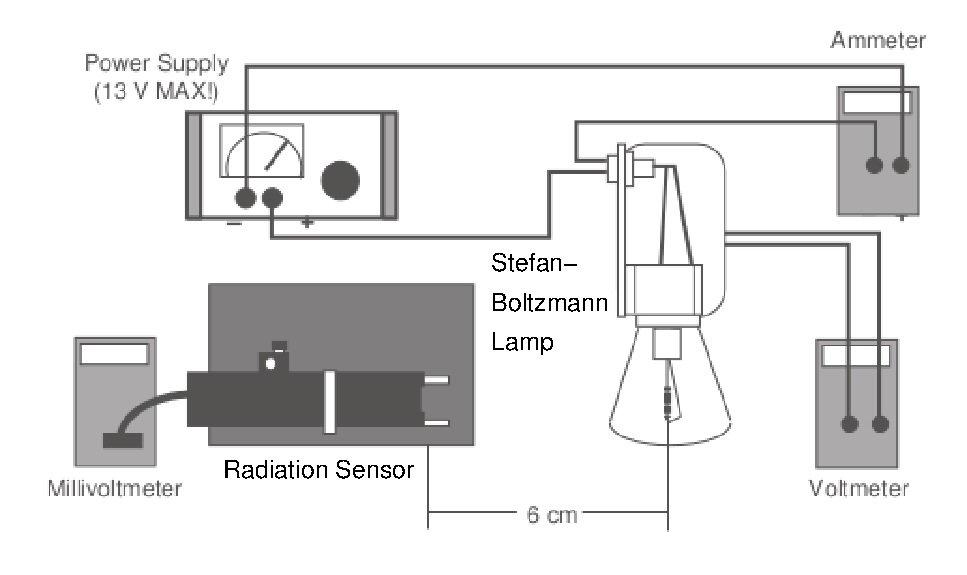
\includegraphics[height=2.5in]{stefansLaw/stefansLawFig1h.eps}
\caption{Equipment setup for Stefan's Law.}\label{setup}
\end{center}
\end{figure}

(c) Use Table \ref{dataTable} to collect your results. Fill the top row with headings 
$V$ (volts), $I$ (Amps), $\mathscr{P}$ (mV), $R$ (ohms), 
$R/R_{rel}$, and $T$ (K).
You can also create this table in {\it Excel}, but make sure you save the file and print a copy
to put in your notebook. 

\begin{table}[hbt]
\begin{center}
\begin{tabular}{|p{0.8in}|p{0.8in}|p{0.8in}|p{0.8in}|p{0.8in}|p{0.8in}|} \hline
\ & \ & \ & \ & \ & \ \\ \hline
\ & \ & \ & \ & \ & \ \\
\ & \ & \ & \ & \ & \ \\
\ & \ & \ & \ & \ & \ \\
\ & \ & \ & \ & \ & \ \\
\ & \ & \ & \ & \ & \ \\
\ & \ & \ & \ & \ & \ \\
\ & \ & \ & \ & \ & \ \\
\ & \ & \ & \ & \ & \ \\
\ & \ & \ & \ & \ & \ \\
\ & \ & \ & \ & \ & \ \\
\ & \ & \ & \ & \ & \ \\
\ & \ & \ & \ & \ & \ \\
\ & \ & \ & \ & \ & \ \\
\ & \ & \ & \ & \ & \ \\
\ & \ & \ & \ & \ & \ \\
\ & \ & \ & \ & \ & \ \\
\ & \ & \ & \ & \ & \ \\ \hline
\end{tabular}
\caption{Data table.}\label{dataTable}
\end{center}
\end{table}

(d) Before turning on the power supply turn the voltage dial all the way down (counterclockwise).
Now turn on the power supply. The voltage reading should be zero.

(e) To get the electrical resistance $R$ of the lamp we will measure the voltage $V$ and the current
$I$ through the lamp and use Ohm's Law $V=IR$ to extract $R$. 
The power $\mathscr{P}$ will be measured as a voltage from the millivoltmeter on the multimeter 
attached to the
radiation sensor.
Set the voltage on the power supply, $V$, to the values in the range $1-13~V$ in steps of 1-2 volts.
At each voltage setting, record the current $I$ from the ammeter, and $\mathscr{P}$, the
reading on the millivoltmeter.

IMPORTANT: Make each radiation sensor reading quickly. Between readings, place sheets
of insulating foam between the lamp and the radiation sensor, with the silvered surface facing the
lamp, so that the temperature of the radiation sensor stays relatively constant.

\textbf{Activity \stepcounter{activity}\arabic{activity}: Extracting Stefan's Law}

(a) Calculate $R$, the resistance of the filament at each of the voltage settings with Ohm's Law $R = V/I$.
 Enter your results in your table.

(b) To determine $T$, the temperature of the
lamp filament at each voltage setting we first need to calculate the relative resistance $R/R_{rel}$.
Do this calculation for each entry in your table and enter the results in your table.
Use this ratio and the calibration curve in Figure \ref{calibration} to find $T$. Enter your results in the table.

\begin{figure}[hbt]
\begin{center}
\includegraphics[height=5.5in]{stefansLaw/stefansLawFig2d.eps}
\caption{Calibration curve to get the filament temperature.}\label{calibration}
\end{center}
\end{figure}

\newpage

(c) Plot $\mathscr{P}$ versus $T$ and fit it. Print your plot and insert it into your notebook.
Record the fit here. Is the plot linear?
Does it follow a power law, {\it i.e.} $\mathscr{P} \propto T^n$?
Does it follow an exponential, {\it i.e.} $\mathscr{P} \propto e^{aT}$?
Record your answer here.
\vspace{1.0cm}

(d) To precisely  determine the mathematical form of the your data, make a semi-log plot, {\it i.e.} plot the common
log of $\mathscr{P}$ versus $T$.  If the data follow an exponential curve, then
they will form a straight line on a semi-log plot.
Show this.
Print your plot and insert it into your notebook.
Is this plot linear?
Do your data lie on an exponential?
\vspace{2.5cm}

(e) Plot the common log of $\mathscr{P}$ versus the common log of $T$ and fit it. 
This plot can be used to determine if your data follow a power law.
Show this too.
Print your plot and insert it into your notebook.
Record the fit here.
\vspace{2.5cm}

(f) How is the slope of the plot you made in part (e) related to the temperature dependence?
\vspace{1.0cm}

(g) How do your results compare with your prediction?
\vspace{1.5cm}

(e) Stefan's Law is usually expressed as $\mathscr{P} = \sigma Ae T^4$ where $\sigma$ is the 
Stefan-Boltzmann constant, $A$ is the surface area of the object, and $e$ is a property of the object 
called the emissivity. 
From your analysis what did you obtain for the exponent on the temperature $T$?
How does it compare with the expected value?
\vspace{1.5cm}

(h) Collect the results from the class, find the average and standard deviation, and record them here.
Do the values agree within experimental uncertainties?
Comment on possible sources of error.
\vspace{1.5cm}

(i) Clearly state an equation for Stefan's Law.

